\documentclass{article}

\usepackage{polski}
\usepackage[letterpaper,top=2cm,bottom=2cm,left=3cm,right=3cm,marginparwidth=1.75cm]{geometry}
\usepackage{amsmath}
\usepackage{graphicx}
\usepackage{algpseudocode}
\usepackage{pgfplots}
\pgfplotsset{compat=1.18}
\usepackage[colorlinks=true, allcolors=blue]{hyperref}
\usepackage{adjustbox} % To resize the table
\usepackage{float} % To resize the table


\title{Obliczenia naukowe lista 2}
\author{Stanisław Tomkowiak}
\date{Listopad 2024}
\begin{document}
\maketitle



\section*{Zadanie 1}
\subsection*{Opis problemu}
Zadanie polegało na minimalnej zmiany danych z zadania 5 z listy pierwszej i porównaniu wyników. Należało usunąć 9 z $x_4=0.5772156649$ oraz 7 z $x_5=0.3010299957$.
\subsection*{Rozwiązanie zadania}
Należy zmienić dane z zadania 5 listy 1.
\subsection*{Wyniki i interpretacja}
\begin{center}
  \begin{tabular}{|c|c|c|}
    \hline
      & Float32 wartości z listy 1   & Float32 wartości z listy 2 \\ [0.5ex]
    \hline
    "w przód"  & -0.4999443  & -0.4999443  \\
    \hline
    "w tył"    & -0.4543457 & -0.4543457 \\
    \hline
    "malejąco" & -0.5       & -0.5  \\
    \hline
    "rosnąco"  & -0.5       & -0.5  \\
    \hline
  \end{tabular}
\end{center}


\begin{center}
  \begin{tabular}{|c|c|c|}
    \hline
      & Float64 wartości z listy 1    & Float64 wartości z listy 2 \\ [0.5ex]
    \hline
    "w przód"  &$1.0251881368296672 \cdot 10^{-10}$  & -0.004296342739891585\\
    \hline
    "w tył"    & $-1.5643308870494366 \cdot 10^{-10}$& -0.004296342998713953  \\
    \hline
    "malejąco" & 0.0     & -0.004296342842280865 \\
    \hline
    "rosnąco"  & 0.0      & -0.004296342842280865 \\
    \hline
  \end{tabular}
\end{center}

Wyniki dla precyzji  \texttt{Float32} są takie same. Wynika to z tego, że zmiany danych wejściowych znajdowały się na 10 miejscu zapisu dziesiętnego. Zatem zmiany pojawiły się w miejscu, które przekracza precyzję arytmetyki. Precyzja ta wynosi $\epsilon =2^{-24} \sim 10^{-7}$.

Wyniki dla precyzji \texttt{Float64} dla sumowania "w przód" i "w tył" zmieniły się z $\sim 10^{-10}$ na $\sim 10^{-3}$. Natomiast dla sumowania "malejąco" i "rosnąco" z 0 na $\sim 10^{-3}$. Spowodowane jest to prawie prostopadłymi wektorami co sprawia, że nawet bardzo małe zmiany danych wpływają znacząco na wynik końcowy. Wskaźnik uwarunkowania dla tego zadania jest bardzo duży.
\subsection*{Wnioski}
Zadanie jest źle uwarunkowane, małe zaburzenia wyników wpływają znacząco na wynik końcowy.

\section*{Zadanie 2}
\subsection*{Opis problemu}
Zadanie polega na zbadaniu funkcji $f(x)=e^x \ln (1+e^{-x})$. Należy wygenerować wykres funkcji w dwóch programach do wizualizacji. Następnie porównać otrzymane wyniki z policzoną granicą:
\[ \lim_{x \rightarrow \infty} e^x \ln (1+e^{-x})=1\]

\subsection*{Wyniki i interpretacja}


\begin{figure}[H]
    \centering
    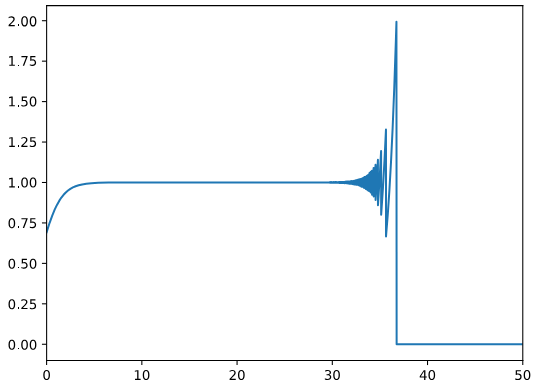
\includegraphics[width=0.8\textwidth, trim = 0 0 0 0, clip]{img/zad2_1.png}
    \caption{Wykres funkcji $f(x)$ wygenerowany w \texttt{pyplot}}
\end{figure}
\begin{figure}[H]
    \centering
    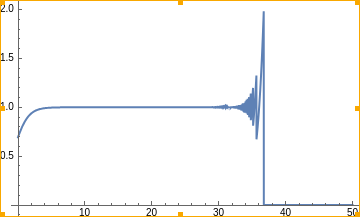
\includegraphics[width=0.8\textwidth, trim = 0 0 0 0, clip]{img/zad2_3.png}
    \caption{Wykres funkcji $f(x)$ wygenerowany w \texttt{Mathematica}}
\end{figure}

Na obu wykresach $37<x$, funkcja  osiąga wartość 0. W obu przypadkach wartość ta dla większych $x$ pozostaje później niezmienna. Jest to wynik niepoprawny ponieważ, granica tej funkcji jest równa 1. Błąd wynika z drugiej części funkcji $\ln (1+e^{-x})$. Fragment $e^{-x}$ w pewnym momencie osiąga wartość zera maszynowego przez co cały logarytm osiąga wartość 0, a przez to całe równanie.  
\subsection*{Wnioski}
Przez granicę precyzji funkcja osiąga błędną granicę.
\section*{Zadanie 3}
\subsection*{Opis problemu oraz sposób rozwiązania} 
Należy rozwiązać równanie $Ax=b$, gdzie A to macierz Hilberta lub losowa macierz kwadratowa o stopniu $n$ z zadanym wskaźnikiem uwarunkowania $c$. Rozwiązać je mamy za pomocą eliminacji Gaussa i $x=A^{-1}b$. Wektor $b$ zadany jest następująco: $b=Ax$, gdzie $x=(1,...,1)^T$. Znamy zatem dokładne rozwiązanie.
\subsection*{Wyniki i interpretacja}
\begin{table}[H]
\centering
\begin{tabular}{|c|c|c|c|}
\hline
\textbf{N} & $\delta_{Gauss}$  & $\delta_{inv}$  & $cond(A)$   \\
\hline
2 & 5.661048867003676e-16 & 1.4043333874306803e-15 & 19.28147006790397 \\
3 & 8.022593772267726e-15 & 0.0 & 524.0567775860644 \\
4 & 4.137409622430382e-14 & 0.0 & 15513.73873892924 \\
5 & 1.6828426299227195e-12 & 3.3544360584359632e-12 & 476607.2502425855 \\
6 & 2.618913302311624e-10 & 2.0163759404347654e-10 & 1.4951058642254734e7 \\
7 & 1.2606867224171548e-8 & 4.713280397232037e-9 & 4.753673567446793e8 \\
8 & 6.124089555723088e-8 & 3.07748390309622e-7 & 1.5257575538060041e10 \\
9 & 3.8751634185032475e-6 & 4.541268303176643e-6 & 4.9315375594102344e11 \\
10 & 8.67039023709691e-5 & 0.0002501493411824886 & 1.602441698742836e13 \\
11 & 0.00015827808158590435 & 0.007618304284315809 & 5.222701316549833e14 \\
12 & 0.13396208372085344 & 0.258994120804705 & 1.7515952300879806e16 \\
13 & 0.11039701117868264 & 5.331275639426837 & 3.1883950689209334e18 \\
14 & 1.4554087127659643 & 8.71499275104814 & 6.200786281355982e17 \\
15 & 4.696668350857427 & 7.344641453111494 & 3.67568286586649e17 \\
16 & 54.15518954564602 & 29.84884207073541 & 7.046389953630175e17 \\
17 & 13.707236683836307 & 10.516942378369349 & 1.249010044779401e18 \\
18 & 10.257619124632317 & 24.762070989128866 & 2.2477642911280653e18 \\
19 & 102.15983486270827 & 109.94550732878284 & 6.472700911391398e18 \\
20 & 108.31777346206205 & 114.34403152557572 & 1.1484020388436145e18 \\
\hline
\end{tabular}
 \caption{Wyniki dla badania macierzy Hilberta rozmiaru $N \times N$}
\end{table}

Wskaźnik uwarunkowania macierzy Hilberta rośnie bardzo szybko. Już dla $n = 13$ wskaźnik uwarunkowania wynosi $6.20\cdot 10^{17}$ co przy precyzji naszej arytmetyki sprawia, że błąd jest bardzo duży. Metoda eliminacji Gaussa jest jednak bardziej skuteczna. Jej błąd względny rośnie wolniej niż metoda $x=A^{-1}b$.   


\begin{table}[H]
\centering
\begin{tabular}{|c|c|c|c|}
\hline
\textbf{N} & \textbf{c} & $\delta_{Gauss}$  & $\delta_{inv}$  \\
\hline
5 & 1.0 & 0.0 & 1.4043333874306804e-16 \\
5 & 10.0 & 2.220446049250313e-16 & 2.808666774861361e-16 \\
5 & 1000.0 & 1.6119276058718354e-15 & 6.513897139161407e-15 \\
5 & 1.0e7 & 2.443504566215332e-10 & 2.224111600609356e-10 \\
5 & 1.0e12 & 1.2766640038565827e-5 & 8.001776490555966e-6 \\
5 & 1.0e16 & 0.45749874095944465 & 0.45970438871083225 \\
10 & 1.0 & 1.6467268631127714e-16 & 3.080743865682491e-16 \\
10 & 10.0 & 3.1006841635969763e-16 & 3.080743865682491e-16 \\
10 & 1000.0 & 1.8675654154580436e-14 & 2.2352514737340923e-14 \\
10 & 1.0e7 & 3.5316264782910544e-10 & 3.725119764302025e-10 \\
10 & 1.0e12 & 1.0377660292087753e-5 & 1.7608144247318942e-5 \\
10 & 1.0e16 & 0.056918623263678886 & 0.04446952959611783 \\
20 & 1.0 & 3.502045386036269e-16 & 4.461660218482181e-16 \\
20 & 10.0 & 3.813741331030777e-16 & 4.736373295277993e-16 \\
20 & 1000.0 & 2.04255692911631e-14 & 2.0390115599110518e-14 \\
20 & 1.0e7 & 2.1724453442256892e-11 & 1.1063284362170502e-10 \\
20 & 1.0e12 & 1.9804529591531784e-5 & 1.7630727486364327e-5 \\
20 & 1.0e16 & 0.12846573399700378 & 0.118301992071668 \\
\hline
\end{tabular}
\caption{Wyniki dla badania macierzy losowej rozmiaru $N \times N$ i i $cond(A)=c$}
\label{tab:dataset}
\end{table}
Macierz losowa zachowuje się lepiej niż Hilberta. Błędy względne dla obu metod mają mniejszą wartość niż w badaniu pierwszym. Błąd można przedstawić jako $\delta \sim c \cdot \epsilon$.

\subsection*{Wnioski}
Im większe są macierze, tym większy błąd względny. Powodem jest złe uwarunkowanie macierzy.  
\section*{Zadanie 4}
\subsection*{Opis problemu}
W zadaniu należało użyć pakietu \texttt{Polynomials} do obliczenia pierwiastków wielomianu:
\[ p(x)=(x-20)(x-19)(x-18)...(x-2)(x-1) \] oraz porównać błędy wyliczonych pierwiastków z prawdziwymi pierwiastkami. Należało także policzyć $p(z_k)$ i $P(z_k)$. 
\subsection*{Rozwiązanie}
Do rozwiązania zadania należało użyć funkcji \texttt{roots} aby wyliczyć pierwiastki wielomianu. Następnie obliczyć dla każdego pierwiastka $|p(z_k)|$ i $|P(z_k)|$ oraz $|z_k-k|$ gdzie k to jest prawdziwy pierwiastek a $z_k$ pierwiastek z użytej funkcji \texttt{roots}. W drugim podpunkcie należało policzyć te same wartości w zaburzonym wielomianie. Od współczynnika -210 należało odjąć $2^{-23}$.
\subsection*{Wyniki i interpretacja}
Wyniki dla oryginalnego wielomianu przedstawiam poniżej: 

\begin{table}[H]
\centering
\begin{tabular}{|c|c|c|c|c|}
\hline
\textbf{$k$} & \textbf{$P(z_k)$} & \textbf{$p(z_k)$} & \textbf{$|z_k - k|$} & \textbf{$z_k$}  \\ \hline
1  & \num{36352.0}       & \num{36626.4254824228}       & \num{3.0109248427834245e-13}       & 0.9999999999996989 \\ \hline
2  & \num{181760.0}      & \num{181303.9336725767}      & \num{2.8318236644508943e-11}       & 2.0000000000283182 \\ \hline
3  & \num{209408.0}      & \num{290172.2858891687}      & \num{4.0790348876384996e-10}       & 2.9999999995920965 \\ \hline
4  & \num{3.106816e6}    & \num{2.04153729027509e6}     & \num{1.626246826091915e-8}         & 3.9999999837375317 \\ \hline
5  & \num{2.4114688e7}   & \num{2.0894625006962176e7}   & \num{6.657697912970661e-7}         & 5.000000665769791 \\ \hline
6  & \num{1.20152064e8}  & \num{1.1250484577562997e8}   & \num{1.0754175226779239e-5}       & 5.999989245824773 \\ \hline
7  & \num{4.80398336e8}  & \num{4.5729086427309465e8}   & \num{0.00010200279300764947}      & 7.000102002793008 \\ \hline
8  & \num{1.682691072e9} & \num{1.5556459377357383e9}   & \num{0.0006441703922384079}       & 7.999355829607762 \\ \hline
9  & \num{4.465326592e9} & \num{4.68781617564839e9}     & \num{0.002915294362052734}        & 9.002915294362053 \\ \hline
10 & \num{1.2707126784e10} & \num{1.2634601896949207e10} & \num{0.009586957518274986}       & 9.990413042481725 \\ \hline
11 & \num{3.5759895552e10} & \num{3.3001284744984142e10} & \num{0.025022932909317674}       & 11.025022932909318 \\ \hline
12 & \num{7.216771584e10} & \num{7.388525665404987e10}   & \num{0.04671674615314281}        & 11.953283253846857 \\ \hline
13 & \num{2.15723629056e11} & \num{1.84762150931442e11}   & \num{0.07431403244734014}        & 13.07431403244734 \\ \hline
14 & \num{3.65383250944e11} & \num{3.551427752842085e11}  & \num{0.08524440819787316}        & 13.914755591802127 \\ \hline
15 & \num{6.13987753472e11} & \num{8.423201558964255e11}  & \num{0.07549379969947623}       & 15.075493799699476 \\ \hline
16 & \num{1.555027751936e12} & \num{1.5707287366258018e12} & \num{0.05371328339202819}       & 15.946286716607972 \\ \hline
17 & \num{3.777623778304e12} & \num{3.3169782238892354e12} & \num{0.025427146237412046}       & 17.025427146237412 \\ \hline
18 & \num{7.199554861056e12} & \num{6.344853141791281e12}  & \num{0.009078647283519814}       & 17.99092135271648 \\ \hline
19 & \num{1.0278376162816e13} & \num{1.2285717366719662e13} & \num{0.0019098182994383706}      & 19.00190981829944 \\ \hline
20 & \num{2.7462952745472e13} & \num{2.318309535271639e13}  & \num{0.00019070876336257925}      & 19.999809291236637 \\ \hline
\end{tabular}
\label{tab:data_table}
\end{table}
Błąd przybliżenia pierwiastków nie jest najgorszy największa różnica jest równa w przybliżeniu równa $0.085$. W znaczącej ilości przypadków był on jednak dużo niższy. Możemy zaobserwować jednak duże odchylenie wartości wielomianu dla wartości bliskiej pierwiastkowi. Nawet dla $z_1$ wartość wielomianu zamiast $0$ jest równa około $36000$. Wynika to z dużej zmienności wartości wielomianu. 

Wyniki dla zaburzonego wielomianu przedstawiam poniżej:
\begin{table}[H]
\centering
\begin{adjustbox}{max width=\textwidth}
\begin{tabular}{|c|c|c|c|c|}
\hline
\textbf{$k$} & \textbf{$P(z_k)$} & \textbf{$p(z_k)$} & \textbf{$z_k - k$} & \textbf{Roots} \\ \hline
1  & \num{20496.0}       & \num{19987.872313406842}       & \num{1.6431300764452317e-13}       & 0.9999999999998357 + 0.0im \\ \hline
2  & \num{339570.0}      & \num{352369.413808796}         & \num{5.503730804434781e-11}        & 2.0000000000550373 + 0.0im \\ \hline
3  & \num{2.2777455e6}   & \num{2.416241558251844e6}      & \num{3.3965799062229962e-9}        & 2.99999999660342 + 0.0im \\ \hline
4  & \num{1.0488020625e7} & \num{1.126370230029202e7}     & \num{8.972436216225788e-8}         & 4.000000089724362 + 0.0im \\ \hline
5  & \num{4.1239073125e7} & \num{4.475744423806907e7}     & \num{1.4261120897529622e-6}        & 4.99999857388791 + 0.0im \\ \hline
6  & \num{1.406328934140625e8} & \num{2.1421031658039317e8} & \num{2.0476673030955794e-5}      & 6.000020476673031 + 0.0im \\ \hline
7  & \num{4.122812662421875e8} & \num{1.7846173427860644e9} & \num{0.00039792957757978087}     & 6.99960207042242 + 0.0im \\ \hline
8  & \num{1.0307901272578125e9} & \num{1.868697217000985e10} & \num{0.007772029099445632}      & 8.007772029099446 + 0.0im \\ \hline
9  & \num{2.1574055781816406e9} & \num{1.3746309775142996e11} & \num{0.0841836320674414}       & 8.915816367932559 + 0.0im \\ \hline
10 & \num{9.384147605647182e9} & \num{1.4900695352000583e12} & \num{0.6519586830380407}       & 10.095455630535774 - 0.6449328236240688im \\ \hline
11 & \num{9.384147605647182e9} & \num{1.4900695352000583e12} & \num{1.1109180272716561}       & 10.095455630535774 + 0.6449328236240688im \\ \hline
12 & \num{3.0012060598372482e10} & \num{3.2962792355717137e13} & \num{1.665281290598479}       & 11.793890586174369 - 1.6524771364075785im \\ \hline
13 & \num{3.0012060598372482e10} & \num{3.2962792355717137e13} & \num{2.0458202766784277}       & 11.793890586174369 + 1.6524771364075785im \\ \hline
14 & \num{2.0030917431984006e11} & \num{9.546022365750218e14} & \num{2.518835871190904}       & 13.992406684487216 - 2.5188244257108443im \\ \hline
15 & \num{2.0030917431984006e11} & \num{9.546022365750218e14} & \num{2.7128805312847097}       & 13.992406684487216 + 2.5188244257108443im \\ \hline
16 & \num{1.1583329328642004e12} & \num{2.742106076928478e16} & \num{2.9060018735375106}       & 16.73074487979267 - 2.812624896721978im \\ \hline
17 & \num{1.1583329328642004e12} & \num{2.742106076928478e16} & \num{2.825483521349608}       & 16.73074487979267 + 2.812624896721978im \\ \hline
18 & \num{5.867381806750561e12} & \num{4.25248587652037e17}   & \num{2.4540214463129764}       & 19.5024423688181 - 1.940331978642903im \\ \hline
19 & \num{5.867381806750561e12} & \num{4.25248587652037e17}   & \num{2.0043294443099486}       & 19.5024423688181 + 1.940331978642903im \\ \hline
20 & \num{9.550552334336e12} & \num{1.3743743559997601e18}   & \num{0.8469102151947894}       & 20.84691021519479 + 0.0im \\ \hline
\end{tabular}
\label{tab:data_table}
\end{adjustbox}
\end{table}

Algorytm znalazł jedynie 10 pierwiastków rzeczywistych. Dla reszty pierwiastki są liczbami zespolonymi. Dodatkowo możemy zauważyć, że błąd między rzeczywistym pierwiastkiem a wyliczonym dzięki funkcji \texttt{roots} jest większy niż w pierwszym podpunkcie. 
\subsection*{Wnioski}
Zadanie obliczenia miejsc zerowych oraz wartości wielomianu  jest źle uwarunkowane. Odjęcie od współczynnika równego $-210$ liczby $2^{-23}$ pokazuje to jeszcze dobitniej. Pierwiastki w znaczącej liczbie mają część urojoną. Dodatkowo wielomian na bardzo małych odcinkach zmienia wartość znacząco. Sprawia to, że podstawiając do wielomianu teoretycznie wyliczony pierwiastek, wynik jest bardzo daleki od 0. Wniosek po analizie tego zadania jest taki, iż zadanie to jest źle uwarunkowane. 



\section*{Zadanie 5}
\subsection*{Opis problemu} 
Rozważamy równanie rekurencyjne (model logistyczny, model wzrostu populacji)
\begin{equation}
    p_{n+1} := p_n + r \cdot p_n \cdot (1 - p_n), \text{ dla } n = 0,1,\dots
    \label{5.rek}
\end{equation}
gdzie $r$ jest pewną daną stałą, $r(1 - p_n)$ jest czynnikiem wzrostu populacji, a $p_0$ jest wielkością populacji stanowiąca procent maksymalnej wielkości populacji dla danego stanu środowiska.

Przeprowadzamy następujące eksperymenty:

1. Dla danych $r=3$ i $p_0=0.01$ wykonać 40 iteracji równania rekurencyjnego w precyzji \texttt{Float32}. Następnie powtórzyć eksperyment jednak po 10 wykonaniu równania obciąć wynik po trzecim miejscu po przecinku. Wykonać do końca iterację to znaczy do 40 iteracji.

2. Dla danych $r=3$ i $p_0=0.01$ wykonać 40 iteracji równania rekurencyjnego w precyzji \texttt{Float32} i \texttt{FLoat64}.
\subsection*{Sposób rozwiązania} 
Podpunkt 1 wykonujemy stosując równanie z treści polecenia, jednak po 10 iteracji stosujemy funkcję \texttt{floor} z wartością $\texttt{digits}=3$. Następnie wykonujemy 40 iteracji bez obcięcia.


Podpunkt 2 wykonujemy przeprowadzając 40 iteracji podanego wzoru w dwóch precyzjach \texttt{Float32} i \texttt{FLoat64}.
\subsection*{Wyniki i interpretacja}

Wyniki dla podpunktu 1:

\begin{table}[H]
\centering
\begin{tabular}{|c|c|c|}
\hline
\textbf{n} & wartości kolejnych iteracji niezaburzone        & wyniki kolejnych iteracji zaburzone        \\ \hline
1          & 0.0397            & 0.0397            \\ \hline
2          & 0.15407173        & 0.15407173        \\ \hline
3          & 0.5450726         & 0.5450726         \\ \hline
4          & 1.2889781         & 1.2889781         \\ \hline
5          & 0.1715188         & 0.1715188         \\ \hline
6          & 0.5978191         & 0.5978191         \\ \hline
7          & 1.3191134         & 1.3191134         \\ \hline
8          & 0.056273222       & 0.056273222       \\ \hline
9          & 0.21559286        & 0.21559286        \\ \hline
10         & 0.7229306         & 0.722             \\ \hline
11         & 1.3238364         & 1.3241479         \\ \hline
12         & 0.037716985       & 0.036488533       \\ \hline
13         & 0.14660023        & 0.1419599         \\ \hline
14         & 0.52192605        & 0.5073818         \\ \hline
15         & 1.2704837         & 1.2572184         \\ \hline
16         & 0.2395482         & 0.28707945        \\ \hline
17         & 0.7860428         & 0.901074          \\ \hline
18         & 1.2905813         & 1.168493          \\ \hline
19         & 0.16552472        & 0.57784426        \\ \hline
20         & 0.5799036         & 1.3096651         \\ \hline
21         & 1.3107499         & 0.092992425       \\ \hline
22         & 0.08880377        & 0.34602693        \\ \hline
23         & 0.33155674        & 1.0249038         \\ \hline
24         & 0.9964373         & 0.94833183        \\ \hline
25         & 1.0070873         & 1.0953275         \\ \hline
26         & 0.9856746         & 0.78208303        \\ \hline
27         & 1.0280352         & 1.2933705         \\ \hline
28         & 0.9415718         & 0.15506029        \\ \hline
29         & 1.1066148         & 0.54811007        \\ \hline
30         & 0.75267017        & 1.2911663         \\ \hline
31         & 1.3111435         & 0.1633339         \\ \hline
32         & 0.08728206        & 0.5733017         \\ \hline
33         & 0.32627377        & 1.3071823         \\ \hline
34         & 0.98573136        & 0.102552414       \\ \hline
35         & 1.0279264         & 0.37865865        \\ \hline
36         & 0.94180745        & 1.0844874         \\ \hline
37         & 1.106226          & 0.8096107         \\ \hline
38         & 0.7536962         & 1.2720344         \\ \hline
39         & 1.3106109         & 0.23392308        \\ \hline
40         & 0.089340806       & 0.7715323         \\ \hline
\end{tabular}
\caption{Wyniki podpunktu 1.}
\label{tab:values}
\end{table}
Wyniki w 40 iteracji są całkowicie od siebie różne. Wynika to z faktu obcięcia wyniku do 3 cyfr po przecinku po 10 iteracji. Wydawałoby się, że taka operacja nie powinna mieć takiego wpływu na wynik końcowy, jednak jest to nie prawda.
\begin{table}[H]
\centering
\begin{tabular}{|c|c|c|}
\hline
\textbf{n} & wyniki dla precyzji \texttt{Float32}        & wyniki dla precyzji\texttt{Float64}               \\ \hline
1          & 0.0397            & 0.039700000000000006      \\ \hline
2          & 0.15407173        & 0.15407173000000005       \\ \hline
3          & 0.5450726         & 0.5450726260444214        \\ \hline
4          & 1.2889781         & 1.2889780011888008        \\ \hline
5          & 0.1715188         & 0.17151914210917463       \\ \hline
6          & 0.5978191         & 0.5978201201070967        \\ \hline
7          & 1.3191134         & 1.3191137924137961        \\ \hline
8          & 0.056273222       & 0.05627157764626167       \\ \hline
9          & 0.21559286        & 0.21558683923264893       \\ \hline
10         & 0.7229306         & 0.7229143011796237        \\ \hline
11         & 1.3238364         & 1.3238419441684237        \\ \hline
12         & 0.037716985       & 0.037695297254799254      \\ \hline
13         & 0.14660023        & 0.14651838271381398       \\ \hline
14         & 0.52192605        & 0.5216706214360409        \\ \hline
15         & 1.2704837         & 1.2702617739357684        \\ \hline
16         & 0.2395482         & 0.24035217277573784       \\ \hline
17         & 0.7860428         & 0.788101190228897         \\ \hline
18         & 1.2905813         & 1.2890943027949757        \\ \hline
19         & 0.16552472        & 0.17108484668450918       \\ \hline
20         & 0.5799036         & 0.5965293124428507        \\ \hline
21         & 1.3107499         & 1.3185755879607823        \\ \hline
22         & 0.08880377        & 0.05837760834476091       \\ \hline
23         & 0.33155674        & 0.22328659791088076       \\ \hline
24         & 0.9964373         & 0.7435756772236771        \\ \hline
25         & 1.0070873         & 1.3155883456187583        \\ \hline
26         & 0.9856746         & 0.07003529709132894       \\ \hline
27         & 1.0280352         & 0.26542635984930363       \\ \hline
28         & 0.9415718         & 0.8503519818886585        \\ \hline
29         & 1.1066148         & 1.2321124482487258        \\ \hline
30         & 0.75267017        & 0.3741465376064961        \\ \hline
31         & 1.3111435         & 1.0766292556171968        \\ \hline
32         & 0.08728206        & 0.8291253603162694        \\ \hline
33         & 0.32627377        & 1.254154851906327         \\ \hline
34         & 0.98573136        & 0.297906229944765         \\ \hline
35         & 1.0279264         & 0.9253805542593504        \\ \hline
36         & 0.94180745        & 1.132534706433374         \\ \hline
37         & 1.106226          & 0.6822342419051102        \\ \hline
38         & 0.7536962         & 1.3326062851369196        \\ \hline
39         & 1.3106109         & 0.0029066069884153833     \\ \hline
40         & 0.089340806       & 0.011601082861106218      \\ \hline
\end{tabular}
\caption{Wyniki podpunktu 2.}
\label{tab:values_precise}
\end{table}
W przypadku podpunktu 2 błąd pojawia się już w pierwszych iteracjach. W 22 iteracji wyniki nie mają żadnej wspólnej liczby w zapisie dziesiętnym. Wynika to z faktu powielania błędu z  kwadratem. W 40 iteracji przez to powielanie jeden wynik jest około 8 razy większy od drugiego.
\subsection*{Wnioski}
Dzięki temu eksperymentowi możemy zauważyć jak duży wpływ mają na wyniki wybrane arytmetyki oraz pozornie nieznaczące zaokrąglenia. Przy wielu iteracjach błąd zaczyna przez to narastać dzięki czemu można tak dobrać dane aby wyniki były kompletnie nie miarodajne. 
\section*{Zadanie 6}
\subsection*{Opis problemu}
Rozważamy równanie rekurencyjne
\[   
    {x_{n+1} := x_n^2 + c}
\] 
dla $n = 0,1,2,\dots$ gdzie $c$ jest pewną daną stałą.

Należy przeprowadzić 40 iteracji równania rekurencyjnego w arytmetyce \texttt{Float64} dla danych:
\begin{enumerate}\label{6.podpunkty}
     \item[A.] $c = -2, x_0 = 1$
    \item[B.] $c = -2, x_0 = 2$
    \item[C.] $c = -2, x_0 = 1.99999999999999$
    \item[D.] $c = -1, x_0 = 1$
    \item[E.] $c = -1, x_0 = -1$
    \item[F.] $c = -1, x_0 = 0.75$
    \item[G.] $c = -1, x_0 = 0.25$
\end{enumerate}


\subsection*{Sposób rozwiązania} 

Należy dla podanych danych w odpowiedniej arytmetyce przeprowadzić 40 iteracji podanego wzoru arytmetycznego.
\subsection*{Wyniki i interpretacja}

Poniżej przedstawiam graficzne wyniki 40 iteracji dla danych A-G:
\begin{figure}[H]
\centering
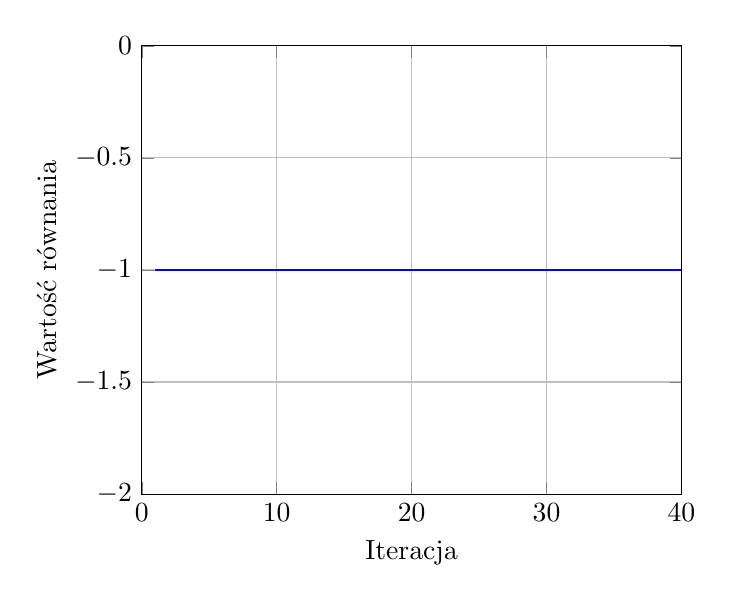
\begin{tikzpicture}
\begin{axis}[
   xlabel={Iteracja},
    ylabel={Wartość równania},
    xmin=0, xmax=40,
    ymin=-2, ymax=0,
    grid=major
]
\addplot[color=blue, mark=none] coordinates {
    (1,-1.0) (2,-1.0) (3,-1.0) (4,-1.0) (5,-1.0) (6,-1.0) (7,-1.0) (8,-1.0)
    (9,-1.0) (10,-1.0) (11,-1.0) (12,-1.0) (13,-1.0) (14,-1.0) (15,-1.0)
    (16,-1.0) (17,-1.0) (18,-1.0) (19,-1.0) (20,-1.0) (21,-1.0) (22,-1.0)
    (23,-1.0) (24,-1.0) (25,-1.0) (26,-1.0) (27,-1.0) (28,-1.0) (29,-1.0)
    (30,-1.0) (31,-1.0) (32,-1.0) (33,-1.0) (34,-1.0) (35,-1.0) (36,-1.0)
    (37,-1.0) (38,-1.0) (39,-1.0) (40,-1.0)
};
\end{axis}
\end{tikzpicture}
\caption{Podpunkt A}
\end{figure}


\begin{figure}[H]
\centering
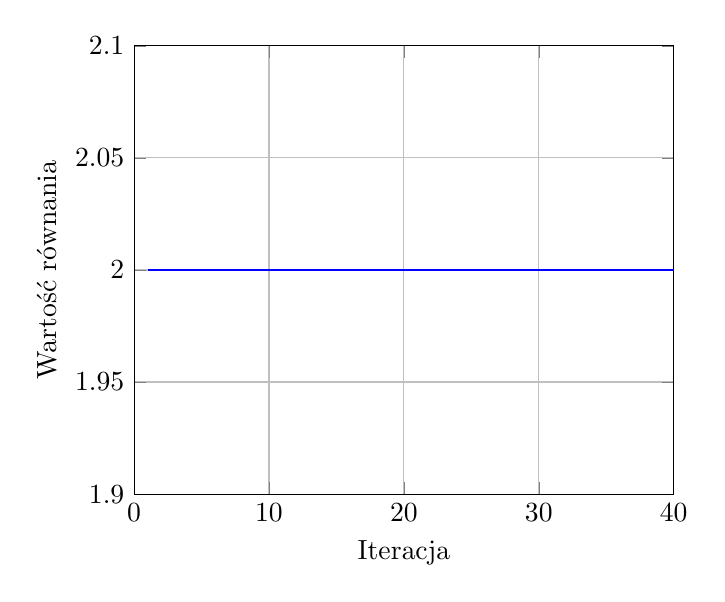
\begin{tikzpicture}
\begin{axis}[
    xlabel={Iteracja},
    ylabel={Wartość równania},
    xmin=0, xmax=40,
    ymin=1.9, ymax=2.1,
    grid=major
]
\addplot[color=blue, mark=none] coordinates {
    (1,2.0) (2,2.0) (3,2.0) (4,2.0) (5,2.0) (6,2.0) (7,2.0) (8,2.0)
    (9,2.0) (10,2.0) (11,2.0) (12,2.0) (13,2.0) (14,2.0) (15,2.0)
    (16,2.0) (17,2.0) (18,2.0) (19,2.0) (20,2.0) (21,2.0) (22,2.0)
    (23,2.0) (24,2.0) (25,2.0) (26,2.0) (27,2.0) (28,2.0) (29,2.0)
    (30,2.0) (31,2.0) (32,2.0) (33,2.0) (34,2.0) (35,2.0) (36,2.0)
    (37,2.0) (38,2.0) (39,2.0) (40,2.0)
};
\end{axis}
\end{tikzpicture}
\caption{Podpunkt B}
\end{figure}

\begin{figure}[H]
\centering
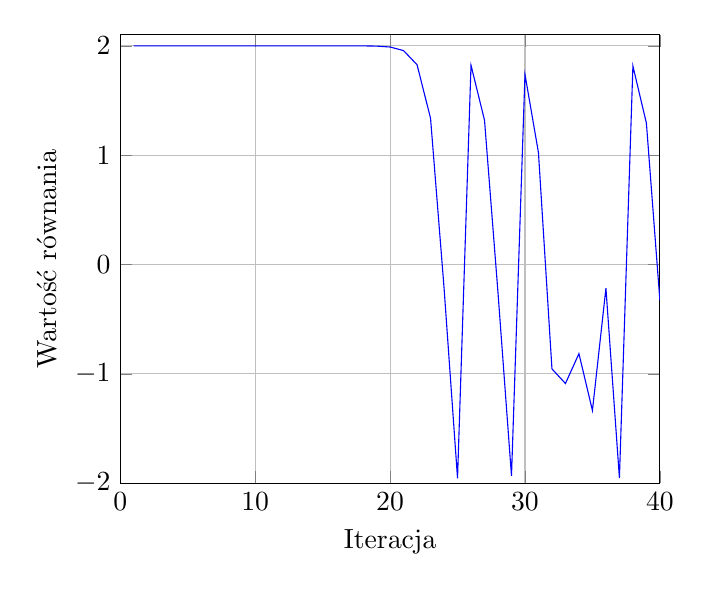
\begin{tikzpicture}
\begin{axis}[
    xlabel={Iteracja},
    ylabel={Wartość równania},
    xmin=0, xmax=40,
    ymin=-2, ymax=2.1,
    grid=major
]
\addplot[color=blue, mark=none] coordinates {
    (1,1.99999999999996) (2,1.9999999999998401) (3,1.9999999999993605)
    (4,1.999999999997442) (5,1.9999999999897682) (6,1.9999999999590727)
    (7,1.999999999836291) (8,1.9999999993451638) (9,1.9999999973806553)
    (10,1.999999989522621) (11,1.9999999580904841) (12,1.9999998323619383)
    (13,1.9999993294477814) (14,1.9999973177915749) (15,1.9999892711734937)
    (16,1.9999570848090826) (17,1.999828341078044) (18,1.9993133937789613)
    (19,1.9972540465439481) (20,1.9890237264361752) (21,1.9562153843260486)
    (22,1.82677862987391) (23,1.3371201625639997) (24,-0.21210967086482313)
    (25,-1.9550094875256163) (26,1.822062096315173) (27,1.319910282828443)
    (28,-0.2578368452837396) (29,-1.9335201612141288) (30,1.7385002138215109)
    (31,1.0223829934574389) (32,-0.9547330146890065) (33,-1.0884848706628412)
    (34,-0.8152006863380978) (35,-1.3354478409938944) (36,-0.21657906398474625)
    (37,-1.953093509043491) (38,1.8145742550678174) (39,1.2926797271549244)
    (40,-0.3289791230026702)
};
\end{axis}
\end{tikzpicture}
\caption{Podpunkt C}
\end{figure}
W przypadku $c=-2$ mamy równanie $x_{n+1} := x_n^2 -2$. Można zauważyć, że punktami stałymi są wartości $x_0=2$ oraz $x_0=1$. Wynik dla tych wartości $x_0$ to odpowiednio 2 i -1. Natomiast dla $x_0=1.99999999999999$ wartości oscylują w przedziale (-2,2). Ostateczny wynik to $-0.3289791230026702$.
\begin{figure}[H]
\centering
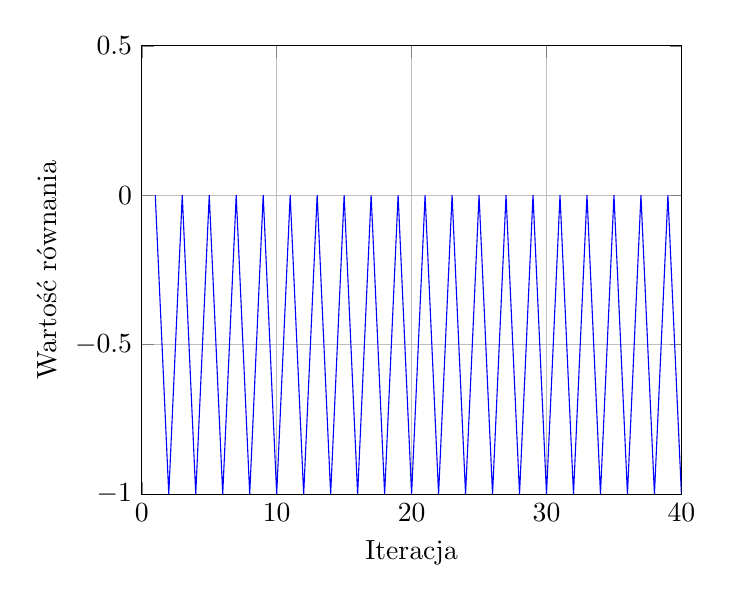
\begin{tikzpicture}
\begin{axis}[
    xlabel={Iteracja},
    ylabel={Wartość równania},
    xmin=0, xmax=40,
    ymin=-1, ymax=0.5,
    grid=major
]
\addplot[color=blue, mark=none] coordinates {
    (1,0.0) (2,-1.0) (3,0.0) (4,-1.0) (5,0.0) (6,-1.0) (7,0.0) (8,-1.0)
    (9,0.0) (10,-1.0) (11,0.0) (12,-1.0) (13,0.0) (14,-1.0) (15,0.0)
    (16,-1.0) (17,0.0) (18,-1.0) (19,0.0) (20,-1.0) (21,0.0) (22,-1.0)
    (23,0.0) (24,-1.0) (25,0.0) (26,-1.0) (27,0.0) (28,-1.0) (29,0.0)
    (30,-1.0) (31,0.0) (32,-1.0) (33,0.0) (34,-1.0) (35,0.0) (36,-1.0)
    (37,0.0) (38,-1.0) (39,0.0) (40,-1.0)
};
\end{axis}
\end{tikzpicture}
\caption{Podpunkt D}
\end{figure}

\begin{figure}[H]
\centering
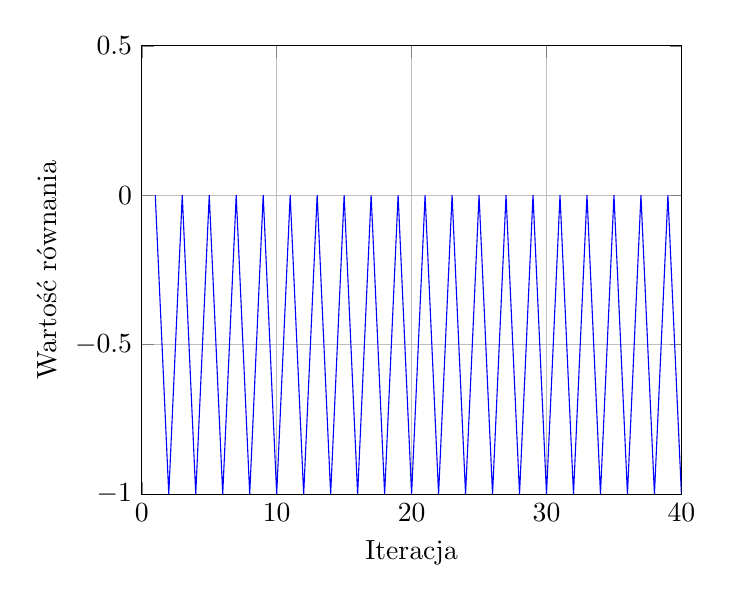
\begin{tikzpicture}
\begin{axis}[
    xlabel={Iteracja},
    ylabel={Wartość równania},
    xmin=0, xmax=40,
    ymin=-1, ymax=0.5,
    grid=major
]
\addplot[color=blue, mark=none] coordinates {
   (1,0.0) (2,-1.0) (3,0.0) (4,-1.0) (5,0.0) (6,-1.0) (7,0.0) (8,-1.0)
    (9,0.0) (10,-1.0) (11,0.0) (12,-1.0) (13,0.0) (14,-1.0) (15,0.0)
    (16,-1.0) (17,0.0) (18,-1.0) (19,0.0) (20,-1.0) (21,0.0) (22,-1.0)
    (23,0.0) (24,-1.0) (25,0.0) (26,-1.0) (27,0.0) (28,-1.0) (29,0.0)
    (30,-1.0) (31,0.0) (32,-1.0) (33,0.0) (34,-1.0) (35,0.0) (36,-1.0)
    (37,0.0) (38,-1.0) (39,0.0) (40,-1.0)
};
\end{axis}
\end{tikzpicture}
\caption{Podpunkt E}
\end{figure}

\begin{figure}[H]
\centering
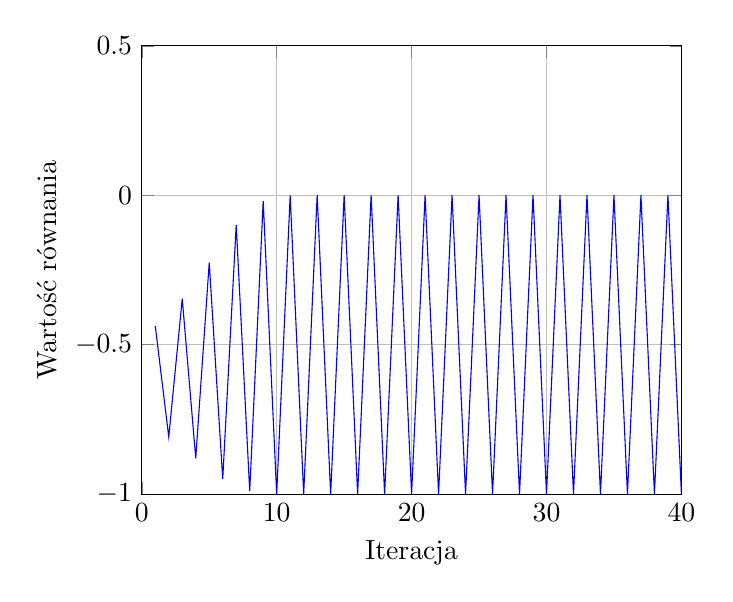
\begin{tikzpicture}
\begin{axis}[
    xlabel={Iteracja},
    ylabel={Wartość równania},
    xmin=0, xmax=40,
    ymin=-1, ymax=0.5,
    grid=major
]
\addplot[color=blue, mark=none] coordinates {
   (1,-0.4375) (2,-0.80859375) (3,-0.3461761474609375)
    (4,-0.8801620749291033) (5,-0.2253147218564956) (6,-0.9492332761147301)
    (7,-0.0989561875164966) (8,-0.9902076729521999) (9,-0.01948876442658909)
    (10,-0.999620188061125) (11,-0.0007594796206411569) (12,-0.9999994231907058)
    (13,-1.1536182557003727e-6) (14,-0.9999999999986692) (15,-2.6616486792363503e-12)
    (16,-1.0) (17,0.0) (18,-1.0) (19,0.0) (20,-1.0) (21,0.0) (22,-1.0)
    (23,0.0) (24,-1.0) (25,0.0) (26,-1.0) (27,0.0) (28,-1.0) (29,0.0)
    (30,-1.0) (31,0.0) (32,-1.0) (33,0.0) (34,-1.0) (35,0.0) (36,-1.0)
    (37,0.0) (38,-1.0) (39,0.0) (40,-1.0)
};
\end{axis}
\end{tikzpicture}
\caption{Podpunkt F}
\end{figure}

\begin{figure}[H]
\centering
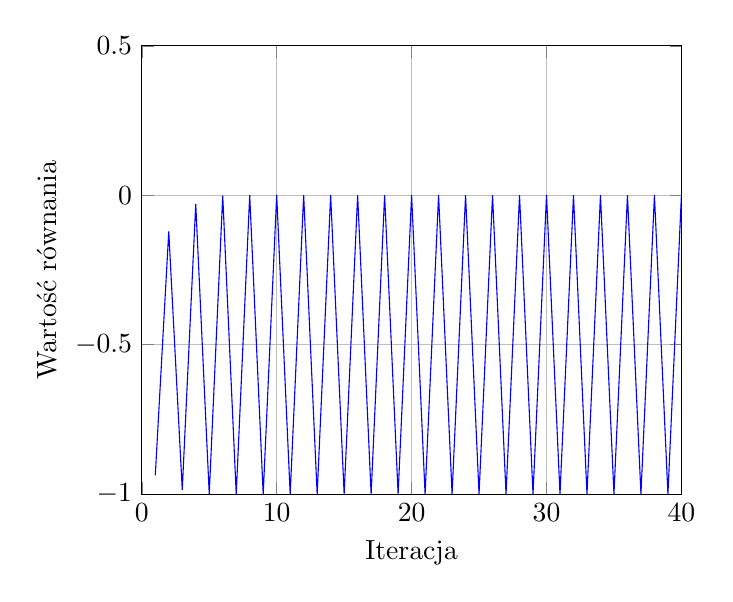
\begin{tikzpicture}
\begin{axis}[
    xlabel={Iteracja},
    ylabel={Wartość równania},
    xmin=0, xmax=40,
    ymin=-1, ymax=0.5,
    grid=major
]
\addplot[color=blue, mark=none] coordinates {
   ((1,-0.9375) (2,-0.12109375) (3,-0.9853363037109375)
    (4,-0.029112368589267135) (5,-0.9991524699951226) (6,-0.0016943417026455965)
    (7,-0.9999971292061947) (8,-5.741579369278327e-6) (9,-0.9999999999670343)
    (10,-6.593148249578462e-11) (11,-1.0) (12,0.0) (13,-1.0) (14,0.0)
    (15,-1.0) (16,0.0) (17,-1.0) (18,0.0) (19,-1.0) (20,0.0) (21,-1.0)
    (22,0.0) (23,-1.0) (24,0.0) (25,-1.0) (26,0.0) (27,-1.0) (28,0.0)
    (29,-1.0) (30,0.0) (31,-1.0) (32,0.0) (33,-1.0) (34,0.0) (35,-1.0)
    (36,0.0) (37,-1.0) (38,0.0) (39,-1.0) (40,0.0)
};
\end{axis}
\end{tikzpicture}
\caption{Podpunkt G}
\end{figure}
W przypadku $c=-1$ mamy równanie $x_{n+1} := x_n^2 -1$. Dla wartości $x_0=1$ oraz $x_0=-1$. Wyniki równania przyjmują naprzemiennie wartości 0 i 1. Ciekawszą próbką są wartości $x_0=0.75$ i $x_0=0.25$, które w rzeczywistości nigdy nie osiągają wartości 0 i -1 jednak przez skończoną precyzję oraz podnoszenie do kwadratu, co sprawia, że przez każde takie mnożenie potrzeba 2 razy więcej cyfr mantysy na wynik, oraz dodawanie -1 do bardzo małej liczby, wartości przyjmują wartości dokładne równe -1 i 0.  
\subsection*{Wnioski}
Zadanie jest źle uwarunkowane podnoszenie do kwadratu oraz odejmowanie od bardzo małych liczb 1 sprawia, że wynik staje się dokładny w przypadkach gdzie taka sytuacja matematycznie nie może się wydarzyć.
\end{document}